\documentclass[]{article}
\usepackage{lmodern}
\usepackage{setspace}
\setstretch{2}
\usepackage{amssymb,amsmath}
\usepackage{ifxetex,ifluatex}
\usepackage{fixltx2e} % provides \textsubscript
\ifnum 0\ifxetex 1\fi\ifluatex 1\fi=0 % if pdftex
  \usepackage[T1]{fontenc}
  \usepackage[utf8]{inputenc}
\else % if luatex or xelatex
  \ifxetex
    \usepackage{mathspec}
  \else
    \usepackage{fontspec}
  \fi
  \defaultfontfeatures{Ligatures=TeX,Scale=MatchLowercase}
\fi
% use upquote if available, for straight quotes in verbatim environments
\IfFileExists{upquote.sty}{\usepackage{upquote}}{}
% use microtype if available
\IfFileExists{microtype.sty}{%
\usepackage{microtype}
\UseMicrotypeSet[protrusion]{basicmath} % disable protrusion for tt fonts
}{}
\usepackage[margin=1in]{geometry}
\usepackage{hyperref}
\hypersetup{unicode=true,
            pdfborder={0 0 0},
            breaklinks=true}
\urlstyle{same}  % don't use monospace font for urls
\usepackage{graphicx,grffile}
\makeatletter
\def\maxwidth{\ifdim\Gin@nat@width>\linewidth\linewidth\else\Gin@nat@width\fi}
\def\maxheight{\ifdim\Gin@nat@height>\textheight\textheight\else\Gin@nat@height\fi}
\makeatother
% Scale images if necessary, so that they will not overflow the page
% margins by default, and it is still possible to overwrite the defaults
% using explicit options in \includegraphics[width, height, ...]{}
\setkeys{Gin}{width=\maxwidth,height=\maxheight,keepaspectratio}
\IfFileExists{parskip.sty}{%
\usepackage{parskip}
}{% else
\setlength{\parindent}{0pt}
\setlength{\parskip}{6pt plus 2pt minus 1pt}
}
\setlength{\emergencystretch}{3em}  % prevent overfull lines
\providecommand{\tightlist}{%
  \setlength{\itemsep}{0pt}\setlength{\parskip}{0pt}}
\setcounter{secnumdepth}{0}
% Redefines (sub)paragraphs to behave more like sections
\ifx\paragraph\undefined\else
\let\oldparagraph\paragraph
\renewcommand{\paragraph}[1]{\oldparagraph{#1}\mbox{}}
\fi
\ifx\subparagraph\undefined\else
\let\oldsubparagraph\subparagraph
\renewcommand{\subparagraph}[1]{\oldsubparagraph{#1}\mbox{}}
\fi

%%% Use protect on footnotes to avoid problems with footnotes in titles
\let\rmarkdownfootnote\footnote%
\def\footnote{\protect\rmarkdownfootnote}

%%% Change title format to be more compact
\usepackage{titling}

% Create subtitle command for use in maketitle
\newcommand{\subtitle}[1]{
  \posttitle{
    \begin{center}\large#1\end{center}
    }
}

\setlength{\droptitle}{-2em}
  \title{}
  \pretitle{\vspace{\droptitle}}
  \posttitle{}
  \author{}
  \preauthor{}\postauthor{}
  \date{}
  \predate{}\postdate{}

\fontsize{12}{20}
\pagenumbering{gobble}

\begin{document}

\subsection{Length-length
relationships}\label{length-length-relationships}

The relationships among total length (TL), fork length (FL), and
pre-caudal length (PCL) in \emph{C. limbatus} for sexes combined were:
\[TL = 1.600 + 1.224 \cdot FL \quad (\textup{ANOVA}: F = 138323, df = 1, 469, p < 0.001) \]
\[TL = 4.206 + 1.340 \cdot PCL \quad (\textup{ANOVA}: F = 33643, df = 1, 295, p < 0.001)\]

\subsection{Depth at capture}\label{depth-at-capture}

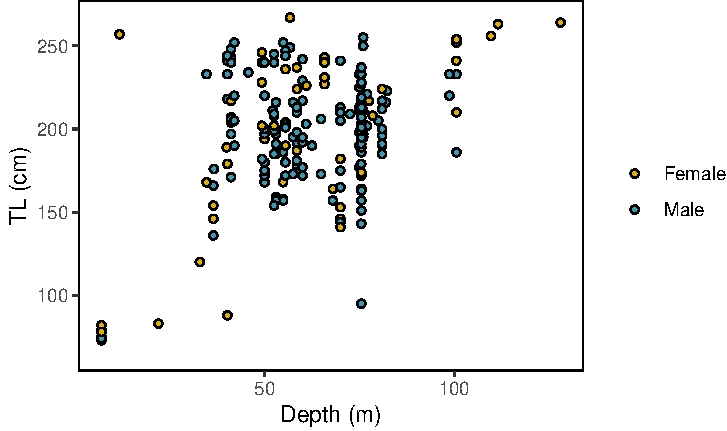
\includegraphics{/Users/alharry/Documents/Manuscripts/limbatus/reports/supplementary_files/figure-latex/figS1-1.pdf}\\
Fig S1. Depth at capture for male and female \emph{C. limbatus} from New
South Wales waters.

\newpage

\subsection{Age and growth}\label{age-and-growth}

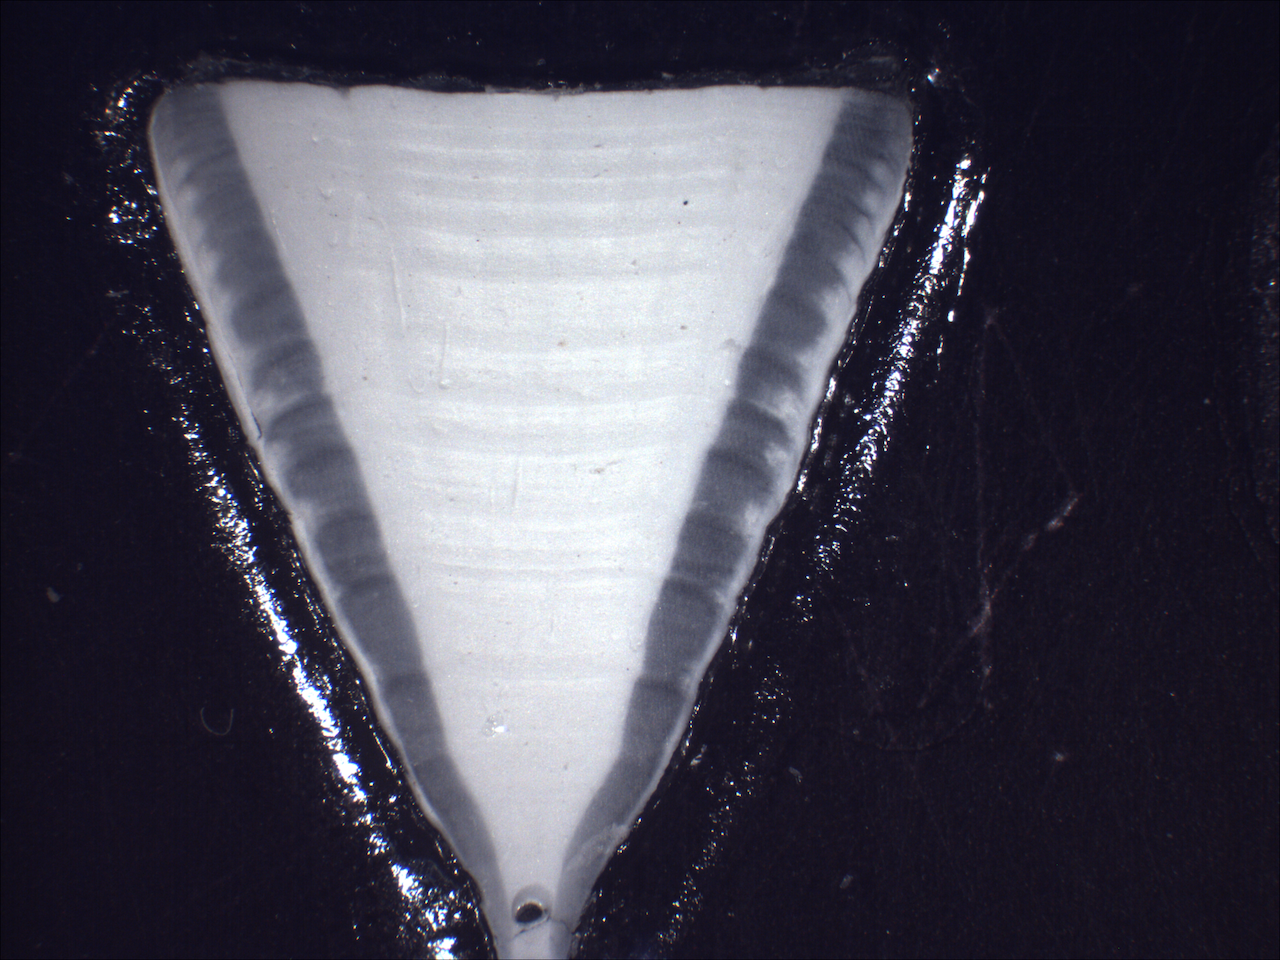
\includegraphics{../data/KH021208-8.png}

Fig. S2. Vertebrae section from a 216 cm male \emph{C. limbatus} with 15
growth zone pairs

\newpage

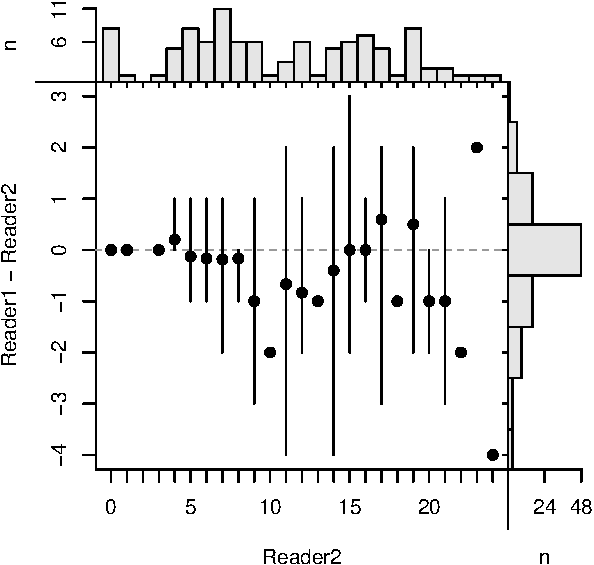
\includegraphics{/Users/alharry/Documents/Manuscripts/limbatus/reports/supplementary_files/figure-latex/figS3-1.pdf}

Fig. S3. Age bias plot showing mean age (plus and minus 95\% confidence
intervals) of Reader 1 relative to those of Reader 2. Sample size of
each age class is denoted at the top of the graph.

\newpage

\subsection{Clasper length}\label{clasper-length}

The male maturation process was investigated by modelling the
development of clasper length, CL, as a function of length using a
modified logistic regression equation
\[ CL(l_i) = f + (g-f)[1+e^{-ln(19)\frac{l_i - CL_{50}}{CL_{95}-CL_{50}}}]^{-1}\cdot e^{\epsilon} \quad \quad \epsilon \sim N(0,\sigma^2)\]
where \emph{f} and \emph{g} are parameters that determine the slope and
intercept, and \(CL_{50}\) and \(CL_{95}\) are the lengths at which
claspers are 50\% and 95\% of their maximum length. The relationship
also has a practical purpose as CL is a useful characteristic for
species identification (Stevens and Wiley 1986; Harry \emph{et al.}
2012).

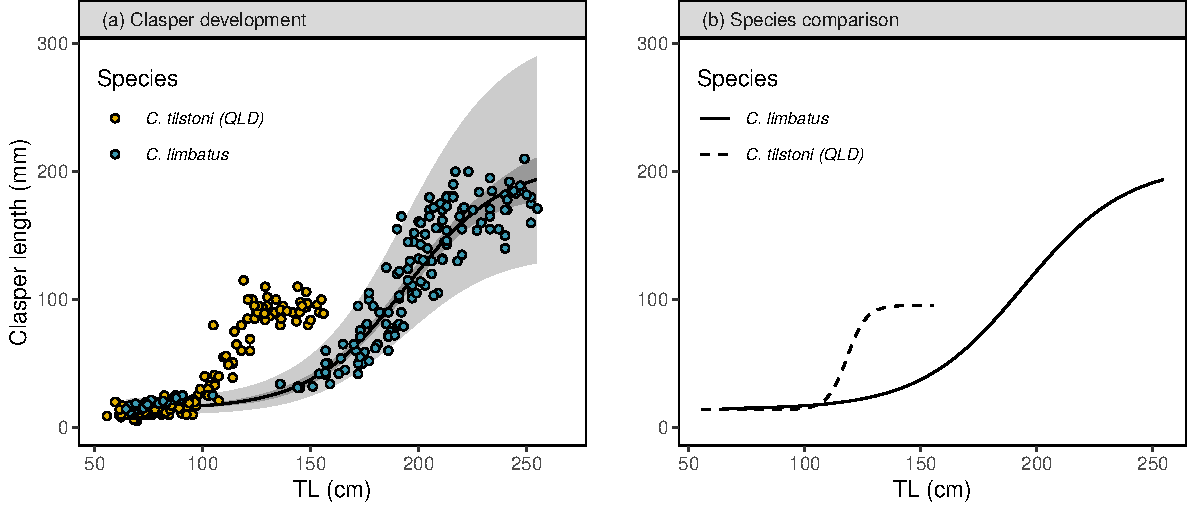
\includegraphics{/Users/alharry/Documents/Manuscripts/limbatus/reports/supplementary_files/figure-latex/figS4-1.pdf}

Fig. S4. Clasper length as a function of length for male \emph{C.
limbatus}. Panel (a) shows non-linear regression model with 95\%
confidence and prediction intervals for \emph{C. limbatus}. Points are
empirical clasper lengths for \emph{C. limbatus} and Qld \emph{C.
tilstoni}. Panel (b) compares the mean relationship between the two
species.

\subsection{Demographic analysis}\label{demographic-analysis}

This section describes aspects of the Monte Carlo simulation used to
investigate sources of uncertainty in the demographic analysis,
including areas where the approach for a specific species / stock
deviates from the general approach described in the methodology.

\subsubsection{Growth parameters}\label{growth-parameters}

Growth parameters for \emph{C. tilstoni} populations based on vertebral
ageing were similar (Davenport and Stevens 1988; Harry \emph{et al.}
2013), although in both cases they were clearly biased as a result of
uncorrected effects of gillnet selectivity. For Qld \emph{C. tilstoni},
a logistic function was chosen to model length at age as the estimated
\(L_\infty\) was closer to observed maximum length of the species. In
the original analysis by Harry \emph{et al.} (2013), this model was fit
with a lognormal variance, and this led to unstable parameter estimates
when attempting to resample random parameters from the
variance-covariance matrix. To provide more reasonabe values for the
Monte Carlo simulation the model was refit with normal variance. For NT
\emph{C. tilstoni}, growth parameters estimated from size mode analysis
were ultimately chosen in favor of those from vertebral ageing as,
again, they were closer to observed maximum length of the species
(Davenport and Stevens 1988). Because the original data were not
available, growth parameters were randomly resampled from a normal
distribution with a CV of 5\%.

\subsubsection{Weight at length}\label{weight-at-length}

No resampling was undertaken on the weight-length parameters for NT
\emph{C. tilstoni} due to the lack of raw data for this species.

\subsubsection{Maturity at length}\label{maturity-at-length}

For NT \emph{C. tilstoni} uncertainty in reproductive output at age was
incorporated by allowing the maternity ogive to shift horizontally over
a range of values by adding a constant to \(A_{50}\) and \(A_{95}\).
Constants were drawn from a random normal distribution with a variance
of 0.5 years (10\% of \(A_{50}\)). The 95\% quantiles of random
\(A_{50}\) values ultimately used in the Monte Carlo simulation were
4.03 to 5.98 years.

\subsubsection{Fecundity}\label{fecundity}

For NT \emph{C. tilstoni} values of fecundity were drawn from a normal
distribution with a mean of 3 (Stevens and Wiley 1986) and a CV of 10\%.
For \emph{C. limbatus} values of fecundity were randomly resampled with
replacement from a vector of mean fecundity values including this and
four other studies (Bass \emph{et al.} 1973; Dudley and Cliff 1993;
Capape \emph{et al.} 2004 ; White 2007).

\subsubsection{Natural mortality}\label{natural-mortality}

\emph{M} was calculated using a constant, size-based method (Then
\emph{et al.} 2015) that required growth parameters \(L_\infty\) and
\emph{K} from the von Bertalanffy equation. This presented a problem for
Qld \emph{C. tilstoni} where a logistic growth model was used to model
growth. Using the values of \(L_\infty\) and \emph{K} from the von
Bertalanffy model in Harry \emph{et al.} (2013) was also deemed
unsuitable because they were strongly biased, and led to unrealistically
small values of \emph{M}. To address this problem, a von Bertalanffy
growth function was re-fit to the length at age data in Harry \emph{et
al.} (2013), constraining \(L_\infty\) to the value in the logistic
growth curve. As per \emph{C. limbatus} and \emph{C. tilstoni}, values
of \(L_\infty\) and \emph{K} used to derive \emph{M} for the Monte Carlo
simulation were then resampled from a multivariate normal distribution
with a mean and covariance matrix obtained from this constrained model.
Noting the high level of uncertainty in \emph{M}, for each simulation
additional variability was added to the calculated value of \emph{M},
drawn from a random normal distribution with a CV of 20\% of \emph{M}.

\newpage

\subsection{\texorpdfstring{Additional discussion points on the ecology
of central eastern Australia \emph{C.
limbatus}}{Additional discussion points on the ecology of central eastern Australia C. limbatus}}\label{additional-discussion-points-on-the-ecology-of-central-eastern-australia-c.-limbatus}

The ecology of \emph{C. limbatus}, like its life history, has
historically been confounded by its co-occurrence and hybridisation with
\emph{C. tilstoni}. Large, adult \emph{C. limbatus}, which are clearly
separable from \emph{C. tilstoni} have been reported in small numbers
throughout northern Australia (Stevens and Wiley 1986; Salini \emph{et
al.} 2007; Johnson \emph{et al.} 2017). Neonate \emph{C. limbatus}, also
easily separable (Harry \emph{et al.} 2012), have been reported from
communal shark nursery areas on both the east and west coasts of
Australia (Simpfendorfer and Milward 1993; White and Potter 2004;
Gutteridge 2011; Taylor and Bennett 2013; Yates \emph{et al.} 2015).

Although the species occurs throughout northern Australia, data from
this study indicate that the central east coast of Australia might be an
area of higher relative abundance for \emph{C. limbatus}. Taylor
\emph{et al.}'s (2013) study of the shark fauna of Moreton Bay showed
\emph{C. limbatus} to be one of the most commonly caught sharks,
suggesting the area would likely meet the formal criteria needed to be
classified as a nursery \emph{sensu} Heupel \emph{et al.} (2007). In
this study we assumed the neonates in Moreton Bay were part of the same
population as those larger sharks sampled off northern NSW. This is not
known definitively, but is a reasonable assumption given the absence of
any other reported parturition areas for \emph{C. limbatus} to the south
and the absence of adults from within Moreton Bay itself (Taylor and
Bennett 2013). Nine small (73 - 83 cm) sharks were also captured during
January and February in 2008 and 2009 from 7m depth off Woody Head
(\(29^\circ 20'S, 153^\circ 21'E\)). Although they were not examined for
the presence of an umbilical scar, all were aged as 0+ and were
therefore likely to have been no more than a few months old. These
individuals provide possible evidence that \emph{C. limbatus}
parturition might also occur in NSW waters.

Little is known about the spatial ecology of \emph{C. limbatus} or
potential linkages between individuals from the central east coast of
Australia in the present study, and those individuals found in tropical
waters further north. Welch \emph{et al.} (2010) investigated the stock
structure of \emph{C. limbatus} off the east coast and identified two
management units separated by the Tropic of Capricorn. Macbeth \emph{et
al.} (2009) also found potential evidence of a seasonal migration in
\emph{C. limbatus}, with the species predominantly caught between
January and June. This suggests a potential northward seasonal migration
during part of the year. Such behaviour would be consistent with that of
some other large carcharhinid sharks (Braccini \emph{et al.} In press)
including populations of \emph{C. limbatus} in the northwest Atlantic
and southwest Indian Ocean (Dudley and Cliff 1993; Kajiura and Tellman
2016).

In keeping with previous studies on hybridisation, no evidence of
intermediate types was found in this study among hybrid sharks (Harry
\emph{et al.} 2012; Johnson \emph{et al.} 2017). All hybrid individuals
showed biological characteristics that were macroscopically similar to
that of purebred \emph{C. limbatus}. The single purebred \emph{C.
tilstoni} identified from NSW using nDNA was a 145cm female captured
from a depth of \textasciitilde{} 42m near the mouth of the Clarence
River, NSW (\(29^\circ 32.99'S, 153^\circ 25.48'E\)). This is the
southernmost record confirmed for this species (excluding individuals
with hybrid ancestry identified solely using mtDNA). The previous
southernmost record was a juvenile \emph{C. tilstoni} from Moreton Bay
identified using a pre-caudal vertebral count (Harry \emph{et al.}
2012).

\subsection*{References}\label{references}
\addcontentsline{toc}{subsection}{References}

\hypertarget{refs}{}
\hypertarget{ref-bass_sharks_1973}{}
Bass AJ, D'Aubrey JD, Kistnasamy N (1973) Sharks of the east coast of
southern Africa. 1. The genus \emph{Carcharhinus (Carcharhinidae)}.
Oceanographic Research Institute, 33. (Durban)

\hypertarget{ref-braccini_dusky_Inpress}{}
Braccini JM, de Lestang S, McAuley RB (In press) Dusky sharks
(\emph{Carcharhinus obscurus}) undertake large-scale migrations between
tropical and temperate ecosystems. \emph{Canadian Journal of Fisheries
and Aquatic Sciences}.
doi:\href{https://doi.org/10.1139/cjfas-2017-0313}{10.1139/cjfas-2017-0313}.

\hypertarget{ref-capape_reproductive_2004}{}
Capape C, Seck AA, Diatta Y, Reynaud C, Hemida F, Zaouali J (2004)
Reproductive biology of the blacktip shark, \emph{Carcharhinus limbatus}
(Chondrichthyes : Carcharhinidae) off west and north African coasts.
\emph{Cybium} \textbf{28}, 275--284.

\hypertarget{ref-davenport_age_1988}{}
Davenport S, Stevens JD (1988) Age and growth of two commercially
important sharks (\emph{Carcharhinus tilstoni} and \emph{C. sorrah})
from Northern Australia. \emph{Australian Journal of Marine and
Freshwater Research} \textbf{39}, 417--433.
doi:\href{https://doi.org/10.1071/MF9880417}{10.1071/MF9880417}.

\hypertarget{ref-dudley_sharks_1993}{}
Dudley SFJ, Cliff G (1993) Sharks caught in the protective gill nets off
Natal, South-Africa 7. The blacktip shark \emph{Carcharhinus limbatus}
(Valenciennes). \emph{South African Journal of Marine Science}
\textbf{13}, 237--254.

\hypertarget{ref-gutteridge_community_2011}{}
Gutteridge AN (2011) Community structure and biology of the
elasmobranchs of Hervey Bay, southeast Queensland, Australia. PhD
Thesis. PhD thesis, University of Queensland, Brisbane.

\hypertarget{ref-harry_comparison_2012}{}
Harry AV, Morgan JAT, Ovenden JR, Tobin AJ, Welch DJ, Simpfendorfer CA
(2012) Comparison of the reproductive ecology of two sympatric blacktip
sharks (\emph{Carcharhinus limbatus} and \emph{Carcharhinus tilstoni})
off north-eastern Australia with species identification inferred from
vertebral counts. \emph{Journal of Fish Biology}.
doi:\href{https://doi.org/10.1111/j.1095-8649.2012.03400.x}{10.1111/j.1095-8649.2012.03400.x}.

\hypertarget{ref-harry_age_2013}{}
Harry AV, Tobin AJ, Simpfendorfer CA (2013) Age, growth and reproductive
biology of the spot-tail shark, \emph{Carcharhinus sorrah}, and the
Australian blacktip shark, \emph{Carcharhinus tilstoni}, from the Great
Barrier Reef World Heritage Area, north-eastern Australia. \emph{Marine
and Freshwater Research} \textbf{64}, 277--293.
doi:\href{https://doi.org/10.1071/MF12142}{10.1071/MF12142}.

\hypertarget{ref-heupel_shark_2007}{}
Heupel MR, Carlson JK, Simpfendorfer CA (2007) Shark nursery areas:
Concepts, definition, characterization and assumptions. \emph{Marine
Ecology Progress Series} \textbf{337}, 287--297.

\hypertarget{ref-johnson_novel_2017}{}
Johnson GJ, Buckworth RC, Lee H, Morgan JAT, Ovenden JR, McMahon CR
(2017) A novel field method to distinguish between cryptic carcharhinid
sharks, Australian blacktip shark \emph{Carcharhinus tilstoni} and
common blacktip shark \emph{C. limbatus}, despite the presence of
hybrids. \emph{Journal of Fish Biology} \textbf{90}, 39--60.
doi:\href{https://doi.org/10.1111/jfb.13102}{10.1111/jfb.13102}.

\hypertarget{ref-kajiura_quantification_2016}{}
Kajiura SM, Tellman SL (2016) Quantification of massive seasonal
aggregations of blacktip sharks (\emph{Carcharhinus limbatus}) in
southeast Florida. \emph{PLOS ONE} \textbf{11}, 1--16.
doi:\href{https://doi.org/10.1371/journal.pone.0150911}{10.1371/journal.pone.0150911}.

\hypertarget{ref-macbeth_observer-based_2009}{}
Macbeth WG, Geraghty PT, Peddemors VM, Gray CA (2009) Observer-based
study of targeted commercial fishing for large shark species in waters
off northern New South Wales. Cronulla Fisheries Research Centre of
Excellence, Industry \& Investment NSW, (Cronulla)

\hypertarget{ref-salini_northern_2007}{}
Salini J, McAuley R, Blaber S, Buckworth R, Chidlow J, Gribble N,
Ovenden J, Peverell S, Pillans R, Stevens J, Tarca C, Walker T (2007)
Northern Australia sharks and rays: The sustainability of target and
bycatch fisheries. Phase 2. CSIRO Marine and Atmospheric Research,
Cleveland,

\hypertarget{ref-simpfendorfer_utilisation_1993}{}
Simpfendorfer CA, Milward NE (1993) Utilisation of a tropical bay as a
nursery area by sharks of the families Charcharinidae and Sphyrinidae.
\emph{Environmental Biology of Fishes} \textbf{37}, 337--345.

\hypertarget{ref-stevens_biology_1986}{}
Stevens JD, Wiley PD (1986) Biology of two commercially important
carcharhinid sharks from northern Australia. \emph{Marine and Freshwater
Research} \textbf{37}, 671--688.
doi:\href{https://doi.org/10.1071/MF9860671}{10.1071/MF9860671}.

\hypertarget{ref-taylor_size_2013}{}
Taylor SM, Bennett MB (2013) Size, sex and seasonal patterns in the
assemblage of Carcharhiniformes in a sub-tropical bay. \emph{Journal of
Fish Biology} \textbf{82}, 228--241.

\hypertarget{ref-then_evaluating_2015}{}
Then AY, Hoenig JM, Hall NG, Hewitt DA (2015) Evaluating the predictive
performance of empirical estimators of natural mortality rate using
information on over 200 fish species. \emph{ICES Journal of Marine
Science: Journal du Conseil} \textbf{72}, 82--92.
doi:\href{https://doi.org/10.1093/icesjms/fsu136}{10.1093/icesjms/fsu136}.

\hypertarget{ref-welch_stock_2010}{}
Welch DJ, Ovenden J, Simpfendorfer C, Tobin A, Morgan JAT, Street R,
White J, Harry AH, Schroeder R, Macbeth WG (2010) Stock structure of
exploitated shark species in north eastern Australia. Report to the
Fisheries Research \& Development Corporation, Project 2007/035. Fishing
\& Fisheries Research Centre Technical Report No. 12, James Cook
University, (Townsville, Australia)

\hypertarget{ref-white_catch_2007}{}
White WT (2007) Catch composition and reproductive biology of whaler
sharks (Carcharhiniformes: Carcharhinidae) caught by fisheries in
Indonesia. \emph{Journal of Fish Biology} \textbf{71}, 1512--1540.
doi:\href{https://doi.org/10.1111/j.1095-8649.2007.01623.x}{10.1111/j.1095-8649.2007.01623.x}.

\hypertarget{ref-white_habitat_2004}{}
White WT, Potter IC (2004) Habitat partitioning among four elasmobranch
species in nearshore, shallow waters of a subtropical embayment in
Western Australia. \emph{Marine Biology} \textbf{145}, 1023--1032.
doi:\href{https://doi.org/10.1007/s00227-004-1386-7}{10.1007/s00227-004-1386-7}.

\hypertarget{ref-yates_spatio-temporal_2015}{}
Yates PM, Heupel MR, Tobin AJ, Simpfendorfer CA (2015) Spatio-Temporal
Occurrence Patterns of Young Sharks in Tropical Coastal Waters.
\emph{Estuaries and Coasts} \textbf{38}, 2019--2030.
doi:\href{https://doi.org/10.1007/s12237-015-9952-4}{10.1007/s12237-015-9952-4}.


\end{document}
